\section{Analysis Overview}
\label{sec:analysis_overview}
The first step to performing a precision measurement of \mH is to ``observe'' many Higgs bosons.
However, production of a Higgs boson is essentially nonexistent in everyday conditions and is still extremely rare even in the high-energy \pp collisions of the LHC (Chapter~\ref{ch:lhc}).
At a center-of-mass energy of 13\TeV, the total inclusive inelastic cross section of two protons colliding is 70\mb.
% TODO: CITE.
Comparing this cross section to the cross section of Higgs boson production $\left( \sigma_{\pp \to \PH} = 59\pb \right)$
% TODO:cite
shows that a Higgs boson is produced in approximately one out of every \emph{billion} \pp collisions---a rare event indeed.
% TODO CITE

To complicate matters further, the Higgs boson has a \emph{very} short mean lifetime of only $1.6 \times \tentotheminus{22}\snd$~\cite{particle_data_group_review_2020}. % TODO:doublecheck.
Thus, the existence of the Higgs boson is not \emph{directly} detected by CMS (Chapter~\ref{ch:cms}) but is instead \emph{inferred} from its stable decay products which enter the various subdetectors.
Among all the fundamental particles so far discovered, the Higgs boson has the second largest mass (approximately 125\GeV),  % TODO: cite best measurement so far.
which gives the scalar boson sufficient energy to decay into at least 9 different final states.
Each decay mode occurs with a different probability---the \emph{branching fraction} (\br)---whose value depends on \mH, as shown in Fig.~\ref{fig:higgs_br}.
The question then becomes, \emph{``Which Higgs boson decay mode is the most useful for measuring \mH?''}
\begin{multiFigure}
	\centering
	% Figures come from:
	% https://twiki.cern.ch/twiki/bin/view/LHCPhysics/LHCHWG?redirectedfrom=LHCPhysics.LHCHXSWG#Higgs_cross_sections_and_decay_b
	\addFigure{0.49}{figures/higgsmassmeas/higgs_BR_80to200GeV.pdf}
	\addFigure{0.49}{figures/higgsmassmeas/higgs_BR_120to130GeV.pdf}
	\captionof{figure}
		[Branching fractions of Higgs boson decays as a function of the Higgs boson mass]
		{The branching fractions of various Higgs boson decays as a function of the Higgs boson mass.
		\;A) Wide range of Higgs boson mass values (80--200\GeV).
		\;B) Narrow range of Higgs boson mass values (120--130\GeV).
	}
	\label{fig:higgs_br}
\end{multiFigure} 
% Real particles enter detectors in CMS which send signals to various electronics.
% Particle Flow algorithm pieces the information together to construct objects out of each event.
% Now, instead of just a deposit of energy in the ECAL and corresponding hits in the silicon tracker, the particle is identified as a newly produced electron.

Owing to its large signal-to-background ratio of approximately 2
% TODO:cite HIG-19-001?
and its relatively rare four-lepton final state, the \hzzfourl decay channel is chosen and is called the \emph{signal process}.
On average, a Higgs boson will decay into two \PZ bosons (one on-shell and the other off-shell) only 2.6\% of the time. % TODO:cite
In turn, each \PZ boson \emph{may} decay into two opposite-sign, same flavor (OSSF) leptons (\ztolplm, where $\ell = \Pe, \Pmu$) on average approximately 6.7\% of the time. % TODO:cite
This signal process then gives rise to four distinct final states: \foure, \fourmu, \twoetwomu, \twomutwoe.
The branching fraction for the overall signal process is then calculated as: % B(Z->ee)=0.033632, B(Z->mumu)=0.033662
\begin{equation*}
    \brof{\hzzfourl} = \brof{\htozz} \left[ \brof{\ztolplm} \right]^2 = 1.8 \times \tentotheminus{3}.
\end{equation*}
Thus, a signal event is expected to be produced only once in about every \emph{trillion} \pp collisions.

The strategy is then to search the \pp collision data collected by CMS for all the detected \hzzfourl events.
The task is not so straightforward;
events in the data are categorized---not by the entire decay process---but by their final state, based on which triggers fired to collect which events.
Section~\ref{sec:analyzed_data} describes the triggers used for this analysis to select events with the \fourl final state found in the corresponding data sets.
For each chosen event, the subdetectors of CMS (Secs.~\ref{sec:tracker}--\ref{sec:muon_sys}) provide a plethora of track and energy-detection information to reconstruct \emph{objects}, which are representations of the underlying particles within the event.
The reconstructed objects are then assembled in a fashion that checks if the decay logic coincides with the signal process of interest: \hzzfourl.
% TODO: Clean up this sentence.
For example, a pair of OSSF lepton-like objects should appear to come from a \PZ-like object---\ie having a nominal mass of approximately 91\GeV and zero net electric charge---instead of, say, appearing to come from a \PH-like object.
Keeping the signal process in mind, then two such \PZ-like objects should be formed and should appear to come from a \PH-like object.
% OSSF-dilepton objects should each appear to come from a \PZ-boson-like object (\eg having a nominal mass of approximately 91\GeV and zero net electric charge)---instead of, say, coming from a Higgs-boson-like object.
All throughout, the reconstructed event must obey all physics conservation laws (energy, momentum, charge, \etc)

The reconstructed objects are often required to pass certain detector selection criteria (\eg $\pt^\Pmu > 5\GeV$).
% This process hinges on the conservation of momentum, since in the longitudinal ($z$) direction the \pp collision has initial and final.
% Specifically, the 
%     - The \PZ boson has a precisely measured mass of TODO a neutral particle, so the two leptons into which it decays should combine to Group two leptons together, 
%     - Form two different pairs of opposite-sign, same-flavor (OSSF) leptons
%     - If it appears that the to select specific hzz4l events (\emph{event selection}).
These criteria are analysis-specific and are collectively called the \emph{event selection} of the analysis.
The event selection for this analysis is described in Sec.~\ref{sec:evt_sel}.
Although the event selection is devised to ideally select only signal events, it is not guaranteed;
there are certain physics process that have exactly the same initial and final states as the signal process.
Such processes ``contaminate'' the collected signal events and are called \emph{background processes}.
Concretely, Fig.~\ref{fig:feyndiag_sig_vs_bkg} shows how identical initial-state gluons can react to produce exactly the same final-state particles, while producing different intermediate particles:
the signal process (\gghzzfourl), initiated by gluon-gluon fusion \vs a background process (\ggzzfourl) which skips the intermediate Higgs boson.
It is imperative for particle physics analyses to maximize the number of collected signal events while minimizing the number of collected background events.
Section~\ref{sec:bkg_estim} discusses the associated background processes and how to estimate the number of events these contribute to the signal region.
\begin{multiFigure}
	\centering
	\addFigure{0.49}{figures/higgsmassmeas/feynman_diag_HZZ4L.png} % TODO: Add gluons to diagram.
	\addFigure{0.49}{figures/higgsmassmeas/feynman_diag_ggZZ4L.png}  % TODO: Fix diagram.
	\captionof{figure}
		[Feynman diagrams for the \gghzzfourl and \ggzzstarfourl processes]
		{Feynman diagrams showing how different physics processes can have the same initial and final states.
		\;A) The signal process \gghzzfourl.
		\;B) An example background process \ggzzfourl.
		}
	\label{fig:feyndiag_sig_vs_bkg}
\end{multiFigure}

%=== How to draw Feynman diagrams in LaTeX.
% Taken from Xunwu's code


%=== Thanks to Dr. Xunwu Zuo for the Feynman diagrams shown in Fig.~\ref{fig:main_higgs_modes}, which shows the major production modes of the Higgs boson. ===%
% Feynman diagrams below don't compile well because the key "horizontal" requires building with LuaTeX.
% \begin{multiFigure}
%     \centering 
%     \captionsetup{justification=centering}
%     \begin{subfigure}[b]{0.45\textwidth} % b for bottom alignment so caption is at the same height
%         \centering
%         \feynmandiagram[horizontal=g1 to t1, horizontal=t2 to h] {
%             g1 [particle = \Pg] -- [gluon] t1,
%             t1 -- [fermion, edge label = \Pqt] t2 -- [fermion, edge label = \Pqt] t3 -- [fermion, edge label = \Pqt] t1,
%             g2 [particle = \Pg] -- [gluon] t3,
%             t2 -- [scalar] h [particle = \PH],
%             g1 -- [draw=none] g2,
%         };

%         \caption*{\ggH}
%     \end{subfigure} 
%     %to put these two diagrams side by side. no empty line in between these two blocks, otherwise it indicates an empty line in the pdf
%     \begin{subfigure}[b]{0.45\textwidth}
%         \centering
%         \feynmandiagram[horizontal=b to h]{
%             q1 [particle = $\Pq_{1}$] -- [fermion] a -- [fermion] aq1 [particle = $\Pq^\prime_{1}$],
%             a -- [boson, edge label = \PV] b -- [boson, edge label = \PV] c,
%             b -- [scalar] h [particle = \PH],
%             aq2 [particle = $\Pq_{2}$] -- [fermion] c -- [fermion] q2 [particle = $\Pq^\prime_{2}$],

%             q1 -- [draw = none] n -- [draw = none] aq2,
%             a -- [draw = none] c,
%             aq1 -- [draw = none] h -- [draw = none] q2,

%         };
%         \caption*{\qqH}
%     \end{subfigure}

%     \begin{subfigure}[b]{0.45\textwidth}
%         \centering
%         \feynmandiagram[horizontal=a to b] {
%             q [particle = \Pq] -- [fermion] a -- [anti fermion] aq [particle = $\Pq^\prime$],
%             a -- [boson, edge label = \PV] b,
%             v [particle = \PV] -- [boson] b -- [scalar] h [particle = \PH],
%         };
%         \caption*{\VH}
%     \end{subfigure}
%     \begin{subfigure}[b]{0.45\textwidth}
%         \centering
%         \feynmandiagram[horizontal=b to h]{
%             g1 [particle = \Pg] -- [gluon] a -- [fermion] t1 [particle = \Pqt],
%             a -- [anti fermion, edge label = \Paqt] b -- [anti fermion, edge label = \Pqt] c,
%             b -- [scalar] h [particle = \PH],
%             g2 [particle = \Pg] -- [gluon] c -- [anti fermion] t2 [particle = \Paqt],

%             g1 -- [draw = none] n -- [draw = none] g2,
%             a -- [draw = none] c,
%             t1 -- [draw = none] h -- [draw = none] t2,
%         };
%         \caption*{\ttH}
%     \end{subfigure}
%     \caption{Main production modes of the Higgs boson.}
%     \label{fig:main_higgs_modes}
% \end{multiFigure}



% \begin{figure*}[!htb]
%     \centering
%     \captionsetup{justification=centering}
%     \begin{subfigure}[b]{0.45\textwidth}
%         \centering
%         \feynmandiagram[horizontal=b to h]{
%             g1 [particle = \Pg] -- [gluon] a -- [fermion] b1 [particle = \Pqb],
%             a -- [anti fermion, edge label = \Paqb] b -- [anti fermion, edge label = \Pqb] c,
%             b -- [scalar] h [particle = \PH],
%             g2 [particle = \Pg] -- [gluon] c -- [anti fermion] b2 [particle = \Paqb],

%             g1 -- [draw = none] n -- [draw = none] g2,
%             a -- [draw = none] c,
%             b1 -- [draw = none] h -- [draw = none] b2,
%         };
%         \caption*{\bbH}
%     \end{subfigure}
%     \begin{subfigure}[b]{0.45\textwidth}
%         \centering
%         \feynmandiagram[horizontal=a to b] {
%             g [particle = \Pg] -- [gluon] a -- [anti fermion] qb [particle = \Pqb],
%             a -- [fermion, edge label = \Pqb] b,
%             w [particle = $\PW^{-}$] -- [boson] b -- [fermion, edge label = \Pqt] th -- [fermion] t [particle = \Pqt],
%             th -- [scalar] h [particle = \PH],
%             t -- [draw = none] h -- [draw = none] w, 
%         };
%         \caption*{\tHW}
%     \end{subfigure}

%     \begin{subfigure}[b]{0.45\textwidth}
%         \centering
%         \feynmandiagram[vertical=a to b] {
%             q [particle = \Pq] -- [fermion] a -- [fermion] aq [particle = \Pq'],
%             a -- [boson, edge label = \PW] b,
%             qb [particle = \Pqb] -- [fermion] b -- [fermion, edge label = \Pqt] c,
%             c -- [scalar] h [particle = \PH],
%             c -- [fermion] t [particle = \Pqt],
%             q -- [draw = none] n -- [draw = none] qb,
%             aq -- [draw = none] h -- [draw = none] c,
%             aq -- [draw = none] h -- [draw = none] t,
%         };
%         \caption*{\tHq}
%     \end{subfigure}
%     \begin{subfigure}[b]{0.45\textwidth}
%         \centering
%         \feynmandiagram[horizontal=b to h]{
%             q1 [particle = \Pq] -- [fermion] a -- [fermion] q2 [particle = $\Pq^\prime$],
%             a -- [boson, edge label = \PW] b -- [boson, edge label = \PW] c,
%             b -- [scalar] h [particle = \PH],
%             qb [particle = \Pqb] -- [fermion] c -- [fermion] qt [particle = \Pqt],

%             q1 -- [draw = none] n -- [draw = none] qb,
%             a -- [draw = none] c,
%             q2 -- [draw = none] h -- [draw = none] qt,
%         };
%         \caption*{\tHq}
%     \end{subfigure}

%     \begin{subfigure}[b]{0.45\textwidth}
%         \centering
%         \feynmandiagram[horizontal=g1 to q1, horizontal=q2 to z] {
%             g1 [particle = \Pg] -- [gluon] q1,
%             q1 -- [fermion, edge label' = \Pq] q2 -- [fermion, edge label' = \Pq] q3 -- [fermion, edge label' = \Pq] q1,
%             g2 [particle = \Pg] -- [gluon] q3,
%             q2 -- [boson, edge label = \PZ] z ,
%             z -- [boson] z2 [particle = \PZ],
%             z -- [scalar] h [particle = \PH],
%             g1 -- [draw=none] g2,
%         };
%         \caption*{\ggZH}
%     \end{subfigure} 
%     \begin{subfigure}[b]{0.45\textwidth}
%         \centering
%         \feynmandiagram[horizontal=t1 to t2] {
%             g1 [particle = \Pg] -- [gluon] t1 -- [fermion, edge label = \Pqt] t2 -- [boson] z [particle = \PZ],
%             g2 [particle = \Pg] -- [gluon] t4 -- [anti fermion, edge label = \Pqt] t3 -- [scalar] h [particle = \PH],
%             t1 -- [anti fermion, edge label = \Pqt] t4,
%             t2 -- [fermion, edge label = \Pqt] t3,
%             g1 -- [draw = none] g2,
%             z -- [draw = none] h,
%         };
%         \caption*{\ggZH}
%     \end{subfigure} 
%     \caption{Examples of minor Higgs boson production modes.}
%     \label{fig:minor_higgs_modes}
% \end{figure*}

Before drawing conclusions from the data themselves, it is necessary for particle physicists to make predictions about their analysis using simulated events or \emph{simulation}.
Such events simulate a specific process (\eg $\pp \to \hzzfourl$), governed by a theoretical model that is programmed mathematically into a software package.
% events from simulated particle physics collisions--- are created by software physicists have created software packages that simulate particle physics collisions,
% the resulting particle transformations using various theoretical frameworks,
% and even the interactions that particles have with the virtual detectors, through which they traverse.
Computer programs like \MGvATNLO and \POWHEG can simulate millions of rare (or even \emph{fictitious}) events in just a single day, whereas gathering the same number of events in CMS data might otherwise take \emph{decades}!
% might otherwise take many years to observe in data.
Furthermore, software can even emulate the process of particles as they travel through simulated detectors.
Programs like \GEANTfour show analysts what to expect as the particles interact with a virtual version of the CMS detector.
Predictions from simulation can then be compared to the truth---\emph{the data}---as a way to check the accuracy of the analysis.
For example, a surplus of events in data where none was expected may lead to the discovery of new particles, as was the case for the discovery of the Higgs boson.
% TODO:cite.
% agreement or deviations in what was expected.
TODO: The simulated events for this analysis are described in Sec.~\ref{sec:sim_samples}.

\emph{So how is the measurement of \mH obtained?}
Since the signal process is \hzzfourl, conservation of energy leads one to expect that $\mfourl \approx \mH$.
Although this is not how the final measurement is obtained, it is a reasonable starting point.
The distribution of \mfourl values reveals that the Higgs boson mass resonance stands well above the distribution of expected background events, as shown in Fig.~\ref{fig:m4l_run2}.
Simulated signal events are then used to predict the \emph{line shape} of this signal peak.
% (Sec.~\ref{sec:signal_model}).
This signal modeling is performed using a double-sided Crystal Ball function to fit the line shape, for various mass points of \mH, in each of the four final states.
% m4l dist Full Run 2.
%%%%%%%%%%%%%%%%%%%%
\begin{multiFigure}
    \centering
    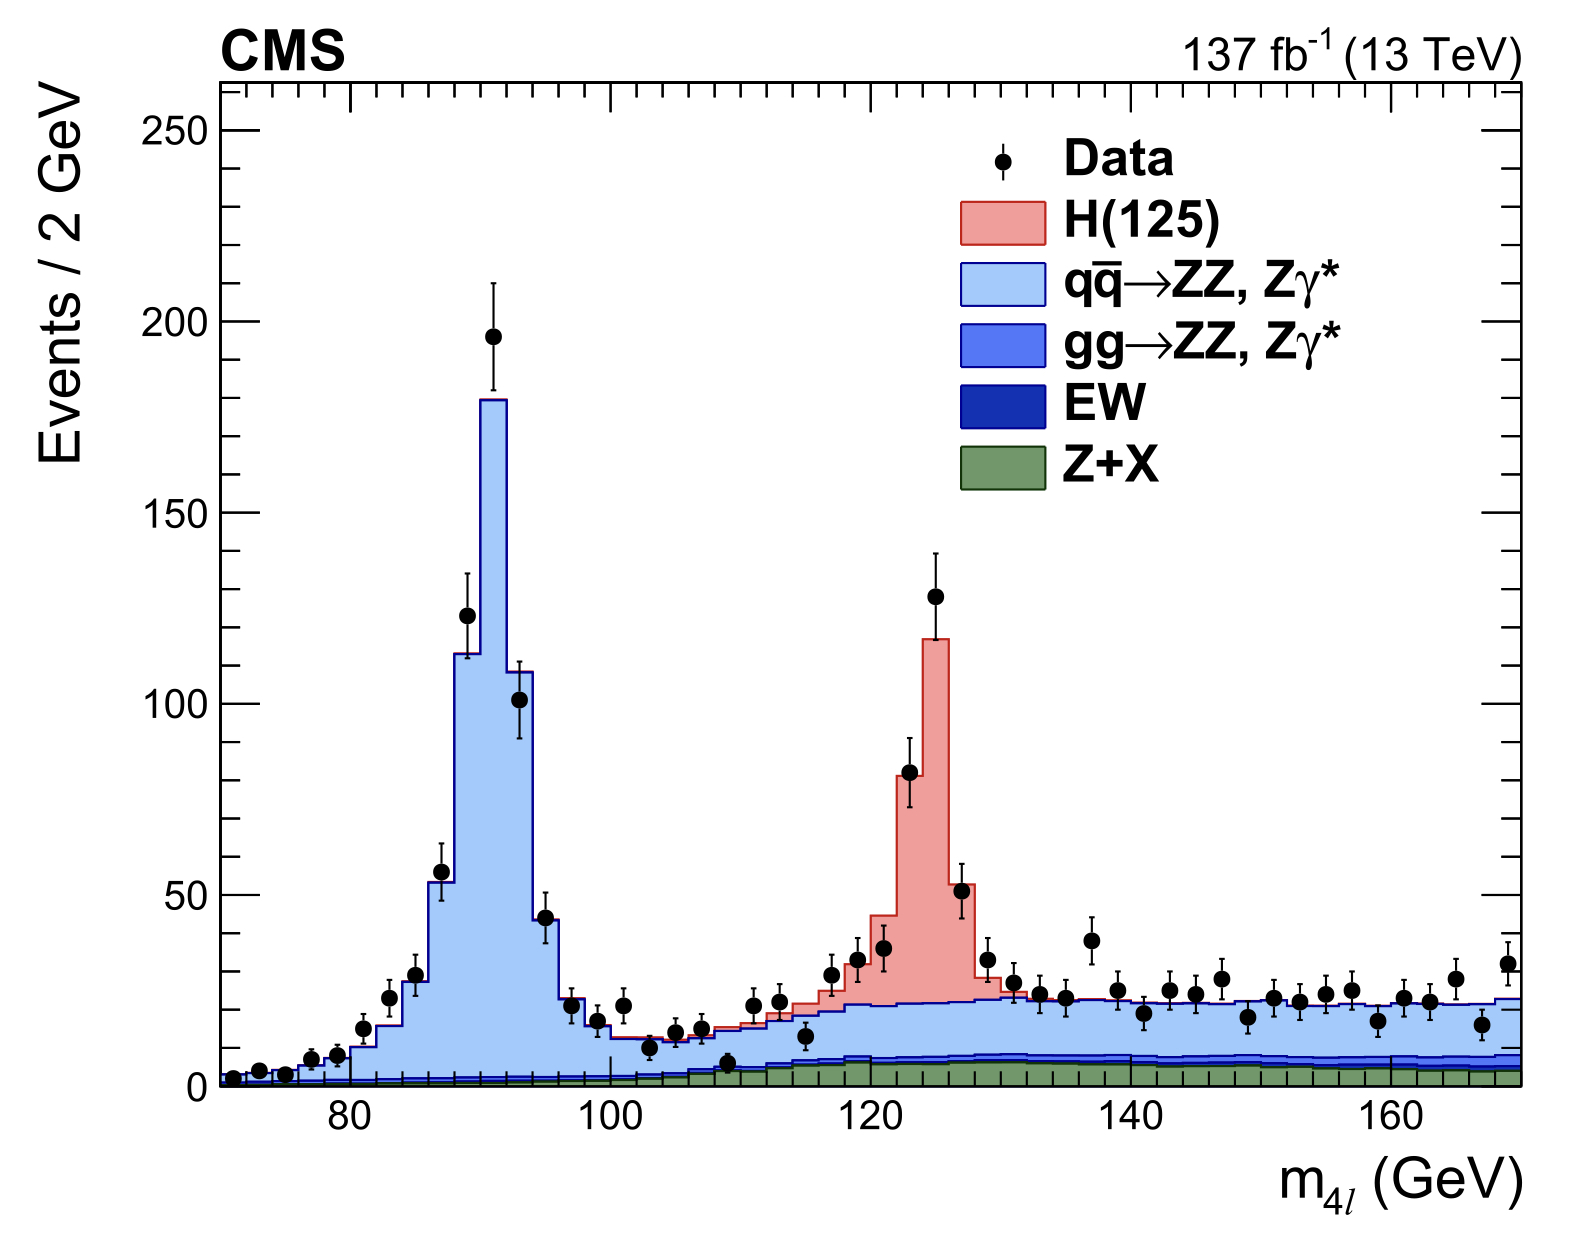
\includegraphics[width=0.8\textwidth,keepaspectratio]{figures/higgsmassmeas/m4l_FullRun2_epjc.jpeg}
	\captionof{figure}
		[Distribution of \mfourl from \hzzfourl events using Full Run 2 data]
		{Distribution of \mfourl from \hzzfourl events using Full Run 2 data.
		Plot taken from~\cite{PhysRevLett.114.191803}. % TODO:cite HIG-19-001 EPJC.
		}
	\label{fig:m4l_run2}
\end{multiFigure}

The precision on the measured value of \mH is improved by implementing several analysis techniques, such as
% \begin{itemize}
% 	\item calculating a per-event matrix element kinematic discriminant
% 	\item deriving correction factors for the uncertainty on \mfourl within various regions of phase space
% 	\item reevaluating the lepton \pt values using a \Zone mass constraint
% 	\item constraining the four muon tracks to the selected vertex (\emph{vertex constraint})
% \end{itemize}
deriving correction factors for the uncertainty on lepton \pt $\left( \ptl \right)$ which gets propagated down to the uncertainty on \mfourl per event,
constraining the four muon tracks to a vertex that is compatible with the beamspot (\emph{vertex+beamspot constraint}),
% TODO: within various regions of which phase space? (pT, eta, phi)?
reevaluating the \ptl values using a \Zone mass constraint per event,
and lastly, splitting events by final state and binning them in relative \mfourl error (\relmfourlerrflat) to avoid an observed correlation between \relmfourlerrflat and \Dkinbkg,
The implementation of these techniques is discussed in Sec.~\ref{sec:techniques}.

% The first technique is called the \Zone mass constraint, which uses the benefit of the mostly on-shell \Zone mass resonance to reevaluate the momenta of the two leptons that built the \Zone, on a per-event basis.
% This improves the overall lepton momentum resolution, thereby improving the resolution of the \mH peak.
% The second technique is per-event mass uncertainty.
% The third technique is vertex constraint.

% is mostly on-shell as opposed to the \Ztwo.
% Z1 significantly on-shell, but Z2 is mostly off-shell.
% 	- Therefore just perform constraint on mZ1.
% 	- Idea is to reevaluate the lepton
% - Per-event 
A matrix element kinematic discriminant $\left( \Dkinbkg \right)$ is calculated on a per-event basis to differentiate signal-like events from background-like events.
% TODO:Incorporate this into techniques above?

Important in any scientific analysis is the careful study of all the associated uncertainties that inherently come with making \emph{any} measurement.
There are two main kinds of uncertainties:
the first is \emph{statistical} uncertainty, which depends on how many data points were collected to make the measurement,
while the second is \emph{systematic} uncertainty, which depends on the precision of the instruments used to make the measurement.
% TODO: Mention theoretical uncertainties?
The systematic uncertainties for this analysis include uncertainties on the integrated luminosity values, lepton identification and reconstruction efficiencies, lepton energy scale and resolution, estimation of the reducible background, and theoretical uncertainties.

% These uncertainties are discussed in Sec.~\ref{sec:syst_uncert}.
All of these ingredients are used in the final measurement, which is obtained via a maximum likelihood fit on the \mfourl spectrum to extract the most likely value of \mH.
The expected results of the precision measurement of \mH are summarized in Sec.~\ref{sec:results}.

% The resolution of the peak 
% Ways to improve the 
% Do likelihood fit.

% TODO: Incorporate the below?
% \textbf{FROM THE AN}
% \begin{itemize}
% 	\item TODO:REWORD First, assess what the expected statistical uncertainty will be on \mH using a 1D $\text{pdf} \left( \mfourl \right)$ on the signal events alone (\ie assuming no background).
% 	\item TODO:REWORD Next, add the vertex constraint in reconstruction of muon \pt.
% 	\item TODO:REWORD Then, use the expected \Zone mass line shape for a scalar Higgs boson to refit the momenta of the leptons originating from the \Zone.
% 	\item Next, we include per-event four-lepton mass uncertainties in the mass measurement. 
% 	Events that are assessed to have better four-lepton mass resolution then acquire higher weight in the mass fit.
% 	\item Add the background and assess how it worsens the expected \mH uncertainties.
% 	\item Introduce the kinematic discriminant $\left( \Dkinbkg \right)$, whose purpose is to discriminate signal events from background events.
% 	This discriminant works on a per-event basis using the four-lepton kinematical observables, instead of directly using the four-lepton mass.
% 	In the Higgs boson mass fit, this gives less weight to events with four-lepton kinematic configurations more typical of background than signal.
% 	\item Finally, add all systematic uncertainties to study how they contribute to, \ie propagate into, the total uncertainty on \mH.
% \end{itemize}




% \begin{table}[!htb]	
% 	\centering
% 	% \captionsetup{justification=justified}
% 	\topcaption{Previous Higgs boson mass measurements made by ATLAS and CMS using the \htofourl decay channel.}
% 	\begin{tabular}{|c|c|c|}
% 		\hline			
% 		Collaboration	&	Mass (GeV) \\
% 		\hline
% 		CMS	            &	125.38 $\pm$ 0.14 \\
% 		ATLAS	        &	124.97 $\pm$ 0.24 \\
% 		\hline			
% 	\end{tabular}
% 	\label{tab:cms_vs_atlas}
% \end{table}
% For reference, Table~\ref{tab:cms_vs_atlas} summarizes the previous Higgs boson mass measurements made by ATLAS and CMS collaborations, using the \htofourl decay channel.
